\FloatBarrier
\section{Evaluation}

\subsection{Method}

The evaluation combines standards-based parameter analysis with policy simulation. Four firmware sizes are considered: 64 KB, 256 KB, 1 MB, and 4 MB. These values span the range from small boot components to ordinary field-update images. For each scheme with signature size $|\sigma|$ and firmware size $|F|$, the package overhead is
\begin{equation}
\text{Overhead}(F,\sigma) = \frac{|\sigma|}{|F|}\times 100\%.
\label{eq:overhead}
\end{equation}

The implementation also estimates the verifier's staging footprint as the sum of public-key bytes, signature bytes, authenticated metadata bytes, and a firmware digest buffer. The runtime experiment performs three trials per scheme over a 47-byte benchmark message and records mean key-generation, signing, and verification latency.

\subsection{Firmware Package Overhead}

Table~\ref{tab:overhead} and Fig.~\ref{fig:overheadplot} show the dependence of package overhead on firmware size. For a 64 KB boot component, ML-DSA-44 contributes 3.6926\% overhead, while SLH-DSA-SHA2-128s contributes 11.9873\%. At 4 MB, these values decrease to 0.0577\% and 0.1873\%, respectively.

\begin{table}[H]
\caption{Signature Overhead Across Firmware Sizes}
\label{tab:overhead}
\centering
\scriptsize
\setlength{\tabcolsep}{2.5pt}
\resizebox{\columnwidth}{!}{%
\begin{tabular}{lccccc}
\toprule
\textbf{Scheme} & \textbf{Sig. (B)} & \textbf{64 KB} & \textbf{256 KB} & \textbf{1 MB} & \textbf{4 MB} \\
\midrule
ECDSA & 64 & 0.0977\% & 0.0244\% & 0.0061\% & 0.0015\% \\
RSA-PSS & 256 & 0.3906\% & 0.0977\% & 0.0244\% & 0.0061\% \\
ML-DSA-44 & 2420 & 3.6926\% & 0.9232\% & 0.2308\% & 0.0577\% \\
ML-DSA-65 & 3309 & 5.0491\% & 1.2623\% & 0.3156\% & 0.0789\% \\
SLH-128s & 7856 & 11.9873\% & 2.9968\% & 0.7492\% & 0.1873\% \\
ECDSA+ML44 & 2484 & 3.7903\% & 0.9476\% & 0.2369\% & 0.0592\% \\
ECDSA+SLH128s & 7920 & 12.0850\% & 3.0212\% & 0.7553\% & 0.1888\% \\
\bottomrule
\end{tabular}
}
\end{table}

For large firmware images, signature size is a secondary cost. For small boot components, the gap between ML-DSA and SLH-DSA remains operationally significant.

\begin{figure}[H]
\centering
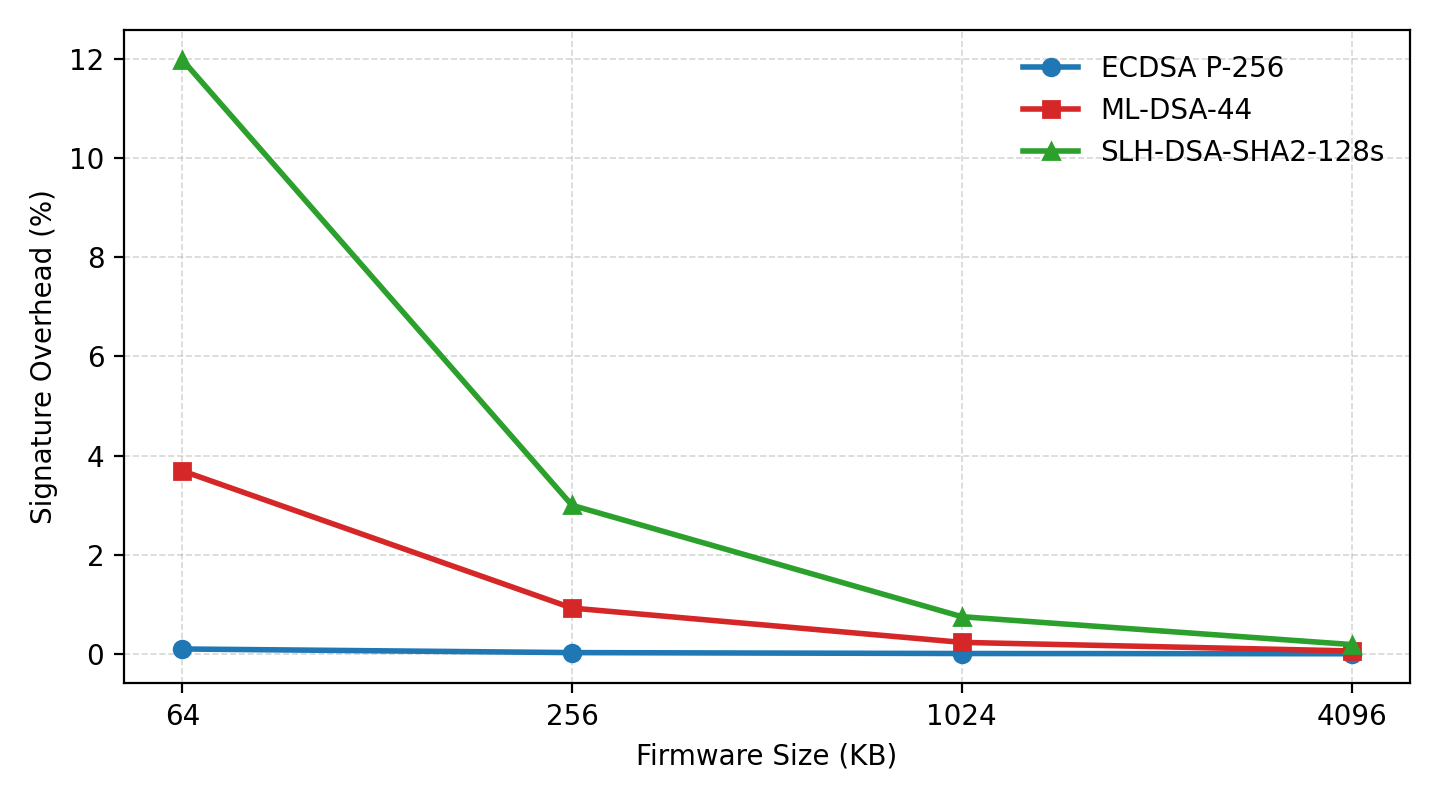
\includegraphics[width=\columnwidth]{../images/firmware_overhead_plot.png}
\caption{Measured overhead trend for representative classical and post-quantum signatures across firmware sizes.}
\label{fig:overheadplot}
\end{figure}

\subsection{Measured PQC Runtime}

Table~\ref{tab:runtime} and Fig.~\ref{fig:runtimeplot} report mean latency from the local PQC backend. ML-DSA-44 completed key generation in 0.299 ms on average, signing in 0.734 ms, and verification in 0.166 ms. In the same environment, the SLH-DSA-SHA2-128s mapping required 206.066 ms for key generation and 1430.190 ms for signing, while verification remained at 1.159 ms.

\begin{table}[H]
\caption{Measured PQC Runtime with the Local \texttt{pqcrypto} Backend}
\label{tab:runtime}
\centering
\scriptsize
\begin{tabular}{p{1.05in}cccc}
\toprule
\textbf{Scheme} & \textbf{Trials} & \textbf{KeyGen} & \textbf{Sign} & \textbf{Verify} \\
\midrule
ML-DSA-44 & 3 & 0.299 & 0.734 & 0.166 \\
SLH-DSA-SHA2-128s & 3 & 206.066 & 1430.190 & 1.159 \\
\bottomrule
\end{tabular}
\end{table}

The local benchmark indicates that ML-DSA is substantially cheaper than SLH-DSA for key generation and signing in this software setting, while both remain fast to verify relative to signing cost.

\begin{figure}[H]
\centering
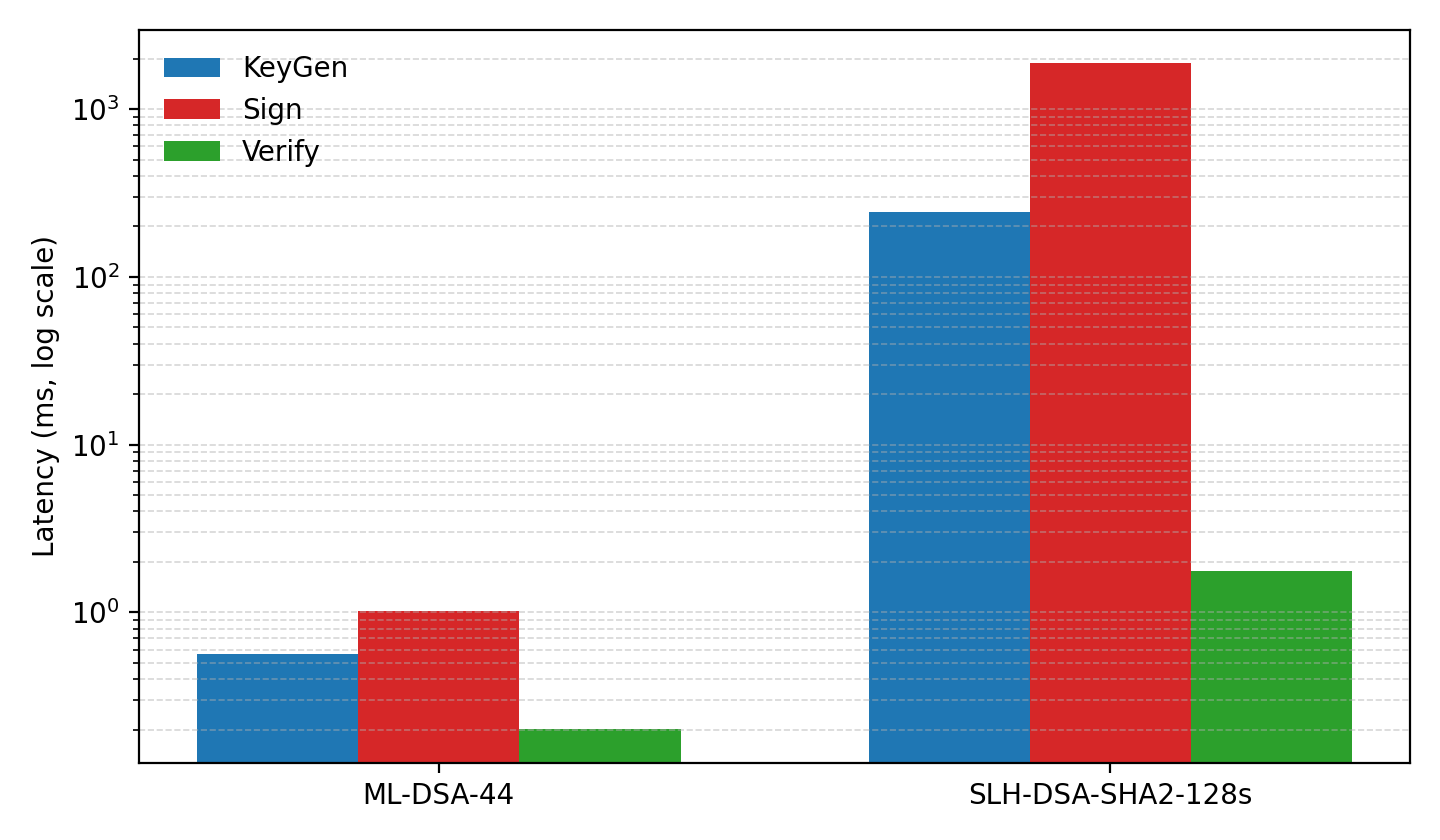
\includegraphics[width=\columnwidth]{../images/pqc_runtime_plot.png}
\caption{Measured PQC runtime. The vertical axis uses logarithmic scale.}
\label{fig:runtimeplot}
\end{figure}

\subsection{Migration Policy Simulation}

The policy simulation evaluates six scenarios across five policies. Table~\ref{tab:policy} shows that the \textit{either-valid} policy accepts a classical-only package after the migration threshold, whereas the version-gated policy rejects it.

\begin{table}[H]
\caption{Policy Simulation Outcomes (\textbf{A} = Accept, \textbf{R} = Reject)}
\label{tab:policy}
\centering
\scriptsize
\setlength{\tabcolsep}{2.5pt}
\resizebox{\columnwidth}{!}{%
\begin{tabular}{p{1.22in}ccccc}
\toprule
\textbf{Scenario} & \textbf{Cls} & \textbf{PQC} & \textbf{Either} & \textbf{Both} & \textbf{V-gated} \\
\midrule
Legacy pre-migration & A & R & A & R & A \\
PQC-only post-migration & R & A & A & R & A \\
Classical-only post-migration & A & R & A & R & R \\
Dual-signed post-migration & A & A & A & A & A \\
Tampered alg. declaration & R & R & R & R & R \\
Rollback package & R & R & R & R & R \\
\bottomrule
\end{tabular}
}
\end{table}

The both-required policy imposes the strongest migration requirement but forces every accepted post-migration package to carry both a classical and a PQ signature. The version-gated policy preserves compatibility before the threshold and removes the classical-only acceptance path after the threshold.

\subsection{Bootloader Suitability}

The bootloader staging values in Table~\ref{tab:profiles} show the same trade-off. SLH-DSA-SHA2-128s has a tiny public key but still requires 8,176 bytes of staged material in the simplified proxy model because the signature dominates. ML-DSA-44 requires 4,020 staged bytes, which is larger than classical baselines but considerably smaller than SLH-DSA.

\subsection{Summary of Findings}

The numerical results support three practical conclusions:
\begin{enumerate}
\item ML-DSA is the most balanced general-purpose PQ option for firmware signing.
\item SLH-DSA is most compelling when conservative security assumptions are worth a significant package-size penalty.
\item Downgrade resistance depends at least as much on verification policy as on the chosen signature algorithm.
\end{enumerate}
